%% LyX 2.2.1 created this file.  For more info, see http://www.lyx.org/.
%% Do not edit unless you really know what you are doing.
%\documentclass[english]{article}
%\usepackage[latin9]{inputenc}

%\usepackage{babel}
%begin{document}

\documentclass[english]{article}
\usepackage[T1]{fontenc}
\usepackage[latin9]{inputenc}
\usepackage[a4paper]{geometry}
\usepackage{amsmath}
\geometry{verbose,tmargin=2cm,bmargin=2cm,lmargin=2cm,rmargin=2cm}
\usepackage{graphicx}
%\usepackage[chapter]{algorithm}
\usepackage{algorithmic}
\newcommand{\norm}[1]{\left\lVert#1\right\rVert}

\DeclareMathOperator*{\argmin}{\arg\!\min}
\DeclareMathOperator*{\argmax}{\arg\!\max}

\makeatletter

%%%%%%%%%%%%%%%%%%%%%%%%%%%%%% LyX specific LaTeX commands.
%% Because html converters don't know tabularnewline
\providecommand{\tabularnewline}{\\}

\makeatother

\usepackage{babel}
\begin{document}

\title{Machine Learning for Computer Vision (EE5177) \\ Programming Assignment 3 : Regression Models \\ Problem \#2}

\author{Akshit Kumar \\ \emph{EE14B127}}

\date{29th March 2017}

\maketitle
\tableofcontents{}

\section{Introduction}

\subsection{Goal}
The goal of the problem is to estimate the head pose of a face using various regression techniques like Linear Regression, Dual Regression, Linear Regression with PCA, Dual Regression with Kernel Trick.
\subsection{Approach}
To estimate the head pose of a face, we employ various regression techniques mentioned above on Histogram of Oriented Gradients (HoG) features.

\subsection{Analysis}
Each regression technique is described here and in conclusion the results obtained from the various regression techniques are evaluted over some test images.

\section{Feature Extraction}
\subsection{Approach}
The actual images are first converted to grayscale images, then they are cropped to only contain the faces and then they are resized to be of the dimension 96px X 108 px. After resizing, the images are used to extract the Histogram of Oriented Gradients feature vectors using the matlab code provided.
\subsection{Sample Cropped Images}
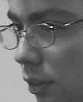
\includegraphics[scale=1]{../cropped_image_1}
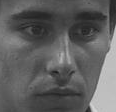
\includegraphics[scale=1]{../cropped_image_2}
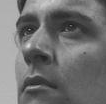
\includegraphics[scale=1]{../cropped_image_3}
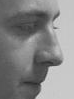
\includegraphics[scale=1]{../cropped_image_4}
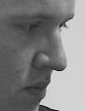
\includegraphics[scale=1]{../cropped_image_5}

\section{Linear Regression using HOG features}
\subsection{ML Estimate}
The ML estimate of the weights can be calculated using 
$$ \phi = (XX^{T})^{-1}Xw $$
where $ X = [x_1,x_2,.........,x_I] $ represents the matrix of HoG features and $w$ represents the world states. 
\subsection{Train and Test Error}
Train RMSE = \textbf{\emph{1.1778e-11}}
\newline
Test RMSE = \textbf{\emph{13.6378}}
\subsection{Analysis}
Clearly the model is \emph{overfitting} the data which is reflected by the fact that the train rmse is too low compared to the test rmse which implies that the model doesn't generalise well. 
Also this method is computationally intensive as $XX^{T}$ is not full rank and not calculating inverse, we need to take a pseudo inverse.

\section{Dual Regression using HOG features}
\subsection{ML Estimate}
The ML estimate of the weights can be calculated using 
$$ \phi = X(X^{T}X)^{-1}w $$
where $ X = [x_1,x_2,.........,x_I] $ represents the matrix of HoG features and $w$ represents the world states. We can show that this estimate is the same as what we would get in the case of linear regression.
\subsection{Train and Test Error}
Train RMSE = \textbf{\emph{3.5667e-11}}
\newline
Test RMSE = \textbf{\emph{13.6378}}
\subsection{Analysis}
Clearly the model is \emph{overfitting} the data which is reflected by the fact that the train rmse is too low compared to the test rmse which implies that the model doesn't generalise well. 
This method performs as well as the Linear regression methos but is computationally less intensive as $X^{T}X$ is full rank and can be easily inverted.

\section{Linear Regression using PCA on HOG features}
\subsection{Choosing the number of components for PCA}
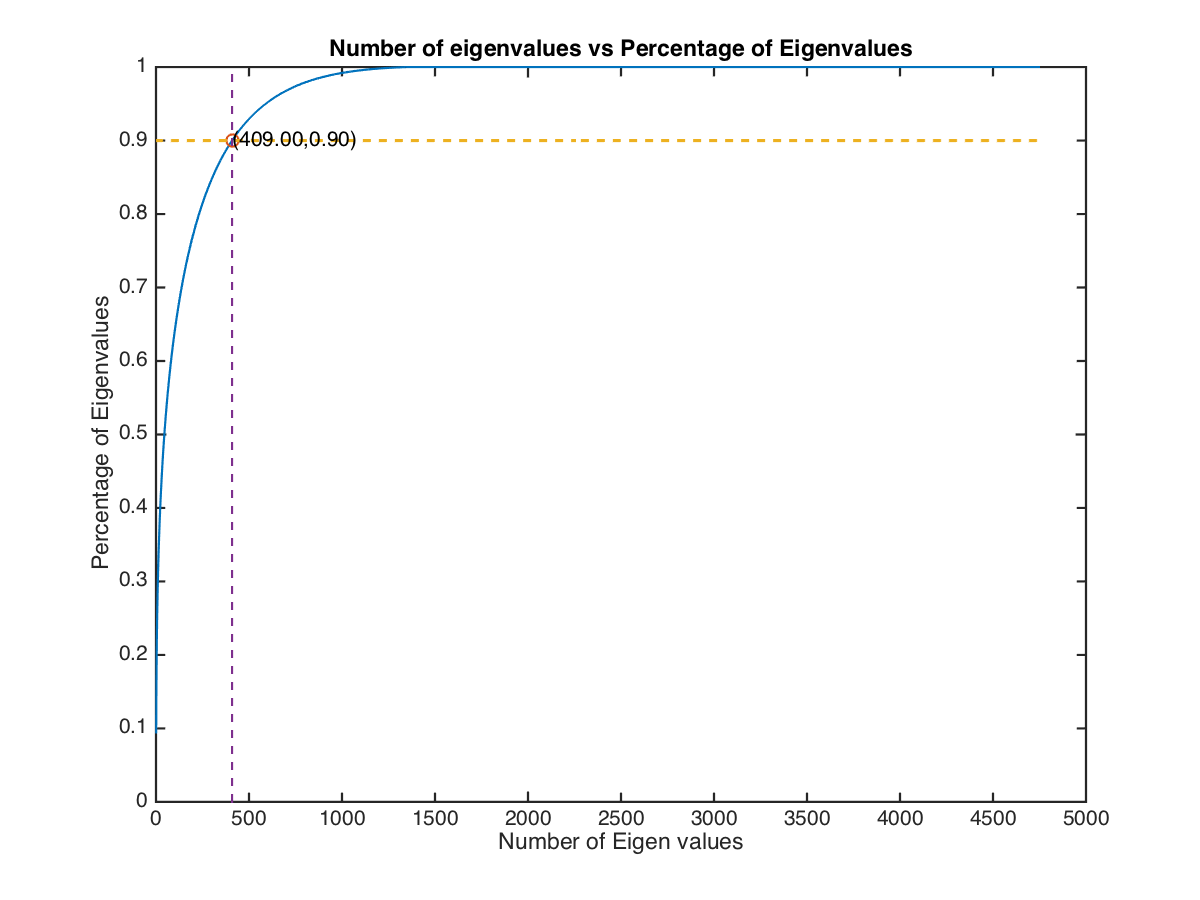
\includegraphics[scale=0.6]{../eigenvalue}
\subsection{Appropriate value of number of components for PCA}
At k = 409, the k largest eigenvalues capture 90\% of the variance. 
\subsection{Train and Test Error}
Train RMSE = \textbf{\emph{7.8429}}
\newline
Test RMSE = \textbf{\emph{10.5769}}
\subsection{Analysis}
Linear Regression using PCA doesn't suffer from overfitting like linear regression and dual regression as PCA tries to capture patterns in data by projecting the data along the plane of highest variance giving simpler models.

\section{Dual Regression with Kernel Trick}
\subsection{RBF Kernel}
In this case we make use of the RBF Kernel, we replace the dot product of 2 vectors with the kernel function as 
$$k[x_i,x_j]=exp[-0.5(\frac{(x_i-x_j)^T(x_i-x_j)}{\lambda^2})]$$
\subsection{Train and Test Error}
\subsubsection{$\lambda_1$ as the minimum pairwise distance}
Train RMSE = \textbf{\emph{3.6863e-13}}
\newline
Test RMSE = \textbf{\emph{12.4462}}
\subsubsection{$\lambda_2$ as the maximum pairwise distance}
Train RMSE = \textbf{\emph{1.4214e-11}}
\newline
Test RMSE = \textbf{\emph{9.6083}}
\subsubsection{$\lambda_3$ as the mean of $\lambda_1$ and $\lambda_2$ }
Train RMSE = \textbf{\emph{2.7439e-12}}
\newline
Test RMSE = \textbf{\emph{8.9713}}
\subsection{Analysis}
Again, all the three models suffer from gross \emph{overfitting}. However this model seems to be performing better than all the other models discussed above as the average value of lambdas gives the least training error and hence generalises best compared to other models discussed above.

\section{Comparison}
\subsection{Comparison of various models in terms of Train and Test RMSE}
\begin{tabular}{|c|c|c|}
\hline
Model & Train RMSE & Test RMSE \\
\hline
Linear Regression & 1.1778e-11 & 13.6378\\
\hline
Dual Regression & 3.5667e-11 & 13.6378\\
\hline
Linear Regression using PCA & 7.8429 & 10.5769\\
\hline
Dual Regression with Kernel Trick ($\lambda_1$) & 3.6863e-13 & 12.4462 \\
\hline
Dual Regression with Kernel Trick ($\lambda_2$) & 1.4214e-11 & 9.6083 \\
\hline
Dual Regression with Kernel Trick ($\lambda_3$) & 2.7439e-12 & 8.9713 \\
\hline
\end{tabular}
\subsection{Analysis}
We can clearly see that Dual Regression with Kernel Trick ($\lambda_3$)seems to perform the best in terms of test rmse metric. We also see that all the models apart from PCA suffer from huge \emph{overfitting} problems and hence it is doesnt generalise well. The reason why Dual Regression with kernel trick does better than other models considered is because these models are able to model the non-linearities in data better which linear models can't really capture. The reason $\lambda_3$ might be doing better than other $\lambda$ values is that it is the mean of the $\lambda_1$ and $\lambda_2$ and is closer to variance than $\lambda_1$ and $\lambda_2$ and hence models the variance better.
\subsection{Pan Angles For Images}
\begin{tabular}{|c|c|c|c|c|c|}
\hline
Model & test/122.jpg & test/337.jpg & test/405.jpg & test/428.jpg & test/550.jpg\\
\hline
Linear Regression Angle & 74.1186 & -51.1052 & -66.0633 & 29.3632 & -6.8440\\
\hline
Dual Regression Angle & 74.1186 & -51.1052 & -66.0633 & 29.3632 & -6.8440\\
\hline
Linear Regression using PCA Angle & 90.2055 & -53.8175 & -74.1713 & 50.6014 & 3.0786 \\
\hline
Dual Regression with Kernel Trick ($\lambda_1$) Angle & 80.4537 & -48.6835 & -72.7297 & 39.0730 & 5.1508 \\
\hline
Dual Regression with Kernel Trick ($\lambda_2$) Angle & 82.1382 & -49.0304 & -72.3169 & 44.5357 & -2.9032 \\
\hline
Dual Regression with Kernel Trick ($\lambda_3$) Angle & 82.8429 & -48.2168 & -74.1274 & 46.2457 & 0.4380 \\
\hline
True Angle & 90 & -45 & -75 & 60 & 0 \\
\hline
\end{tabular}
\subsection{Analysis on Sample Test Images}
From the sample test images, we can clearly see that PCA and Dual regression with kernel trick ($\lambda_3$) seems to be best models for estimation of the head pose angle. Also linear and dual regression perform very badly in estimation which is expected as these models don't capture the variance and non-linearities in the data well.

\end{document}
